%% Bemærk:
%%          Resten af rapporten følger en stil hvor indledninger skrives
%%          med \sffamlily-typen. Denne stil bør også følges her.
%%
{\sffamily
I vores region detektor sætter vi en værdi for hvor stor en region skal
være få at blive tage i betrakting, i dette sektion vil vi hurtigt test,
hvor stor en regionen skal være for at vi vil tage den med. problemet
med få små regioner er illustret i maleri \ref{alt_med} hvor alle de
gråne kasser er en region som vores naive algoritme mener er
interessante, og da alle regioner tage med, bliver 939 regioner godtaget
til at ligge i snittet. 
}

\begin{figure}[¡h]
    \setlength\fboxsep{0pt}
    \setlength\fboxrule{0.5pt}
    \begin{center}
        \fbox{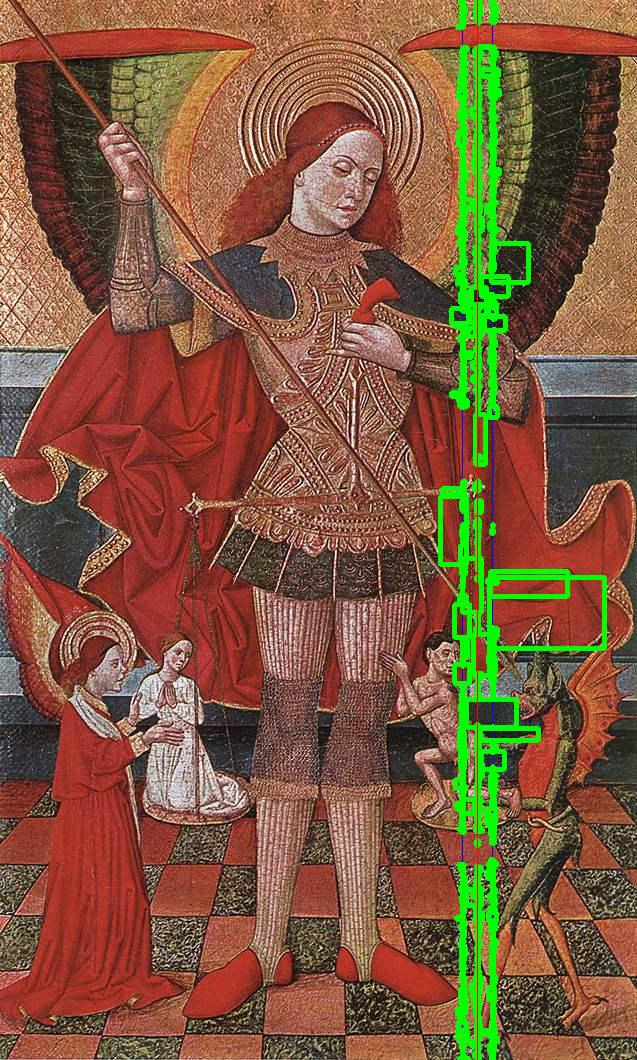
\includegraphics[angle=0,width=0.45\textwidth]{afsnit/afprovning/billeder/stoerelse/alt_med.png}}
    \end{center}
    \caption{Maleri hvor alle størrelse regioner er godtaget, der er fundet 939 intrasante regioner}
\end{figure}
For at teste hvilken størrelse vi gerne vil godtage er der fremstilet et
testbilledet \ref{original_stoerelse} hvor 9 regioner er opstillet så de
alle ligger i sammen snit. Dem øvereste regioner er den minste, og så
stiger regioners størrelse gradvis ned af i billedet.

I vær at de andre 5 testbilleder i figur \ref{stoerelse_sammenlining} er
tærskelværdierne gradvis sat op. Vi mener at der bliver taget for mange
regioner med i billedet \ref{0,0}, \ref{0,005}, \ref{0,001} og
\ref{0,0015}. I billedet \ref{0,002} bliver der taget store nok
regioner, og vi har derfor valt at sætte tærskelværdien til $0.002$
 
\begin{figure}[!h]
    \setlength\fboxsep{0pt}
    \setlength\fboxrule{0.5pt}
    \centering
    \subfloat[original]{
        \fbox{
\includegraphics[angle=0,width=0.45\textwidth]{afsnit/afprovning/billeder/stoerelse/stoerelse.png}}
       \label{original_stoerelse}}
    \subfloat[tærskelværdi sat til 0]{
        \fbox{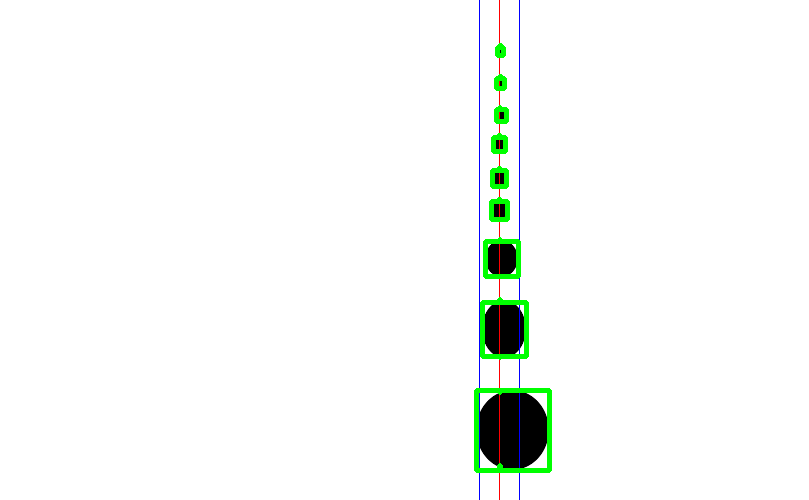
\includegraphics[angle=0,width=0.45\textwidth]{afsnit/afprovning/billeder/stoerelse/0.png}}
       \label{0,0}}\\
    \subfloat[tærskelværdi sat til 0.0005]{
        \fbox{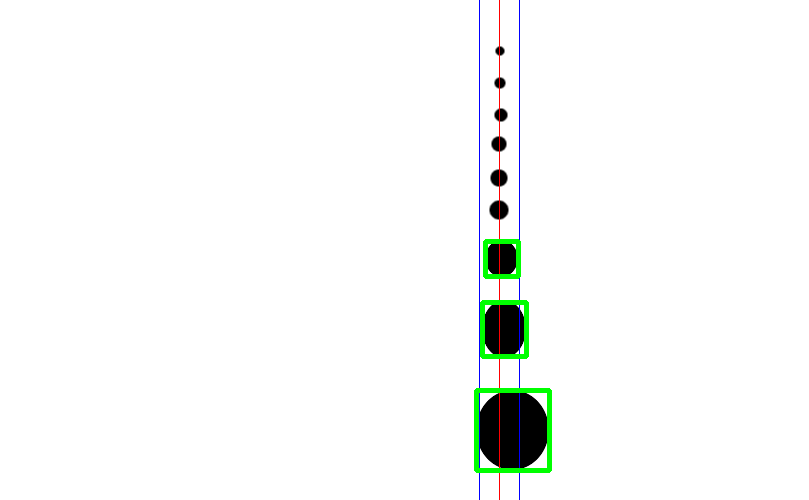
\includegraphics[angle=0,width=0.45\textwidth]{afsnit/afprovning/billeder/stoerelse/0,0005.png}}
       \label{0,005}}
    \subfloat[tærskelværdi sat til 0.001]{
        \fbox{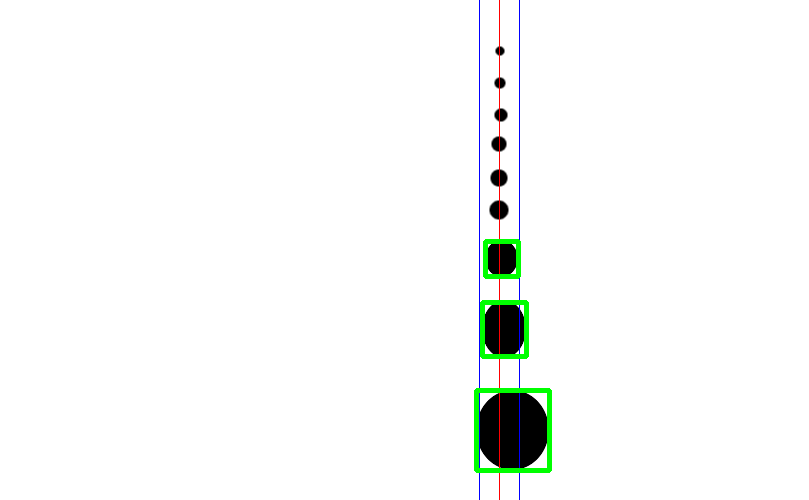
\includegraphics[angle=0,width=0.45\textwidth]{afsnit/afprovning/billeder/stoerelse/0,001.png}}
       \label{0,001}}\\
    \subfloat[tærskelværdi sat til 0.0015]{
        \fbox{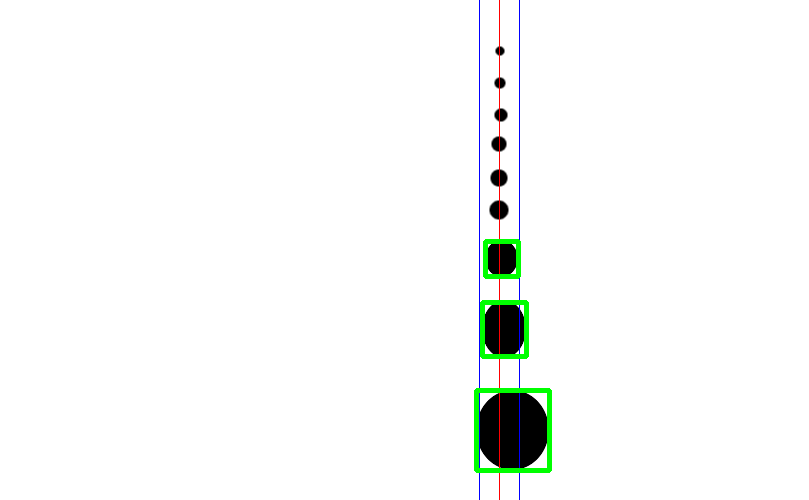
\includegraphics[angle=0,width=0.45\textwidth]{afsnit/afprovning/billeder/stoerelse/0,0015.png}}
       \label{0,0015}}
    \subfloat[tærskelværdi sat til 0.002]{
        \fbox{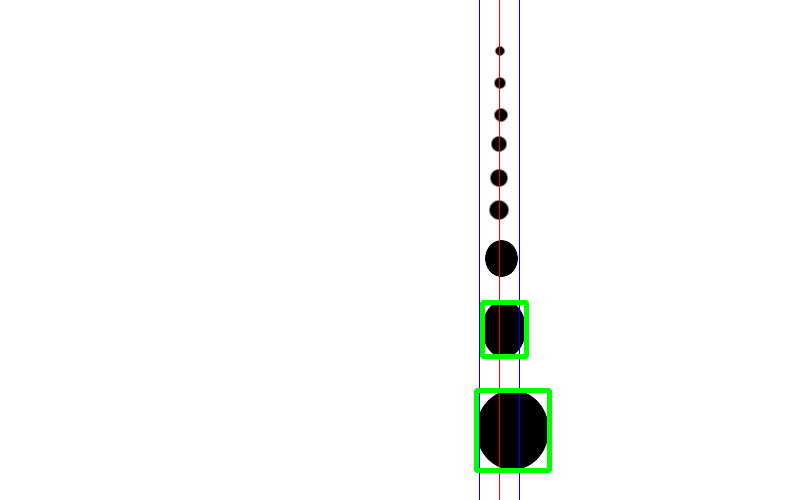
\includegraphics[angle=0,width=0.45\textwidth]{afsnit/afprovning/billeder/stoerelse/0,002.png}}
       \label{0,002}}
    \caption{Testbilledet med 9 regioner som bliver støre og støre, hvor den originale billedet samt 5 forskellige tærskelværdier er afbilledet}
    \label{stoerelse_sammenlining}
\end{figure} 
